\section{Persistent and Situated Agent Lifecycle}
\label{sec:agent-lifecycle}

GAWorld v2 represents an agent as a continuing participant in a shared
simulation, not as an isolated chat session.  The representation separates
relatively stable profile material, mutable runtime state, and artifacts
accumulated over simulated time.  Figure~\ref{fig:agent-lifecycle} shows the
connected per-tick control path, including v2's addition of a personality
pluggable and the indoor-room resolution that occurs after movement.

\begin{figure}[t]
  \centering
  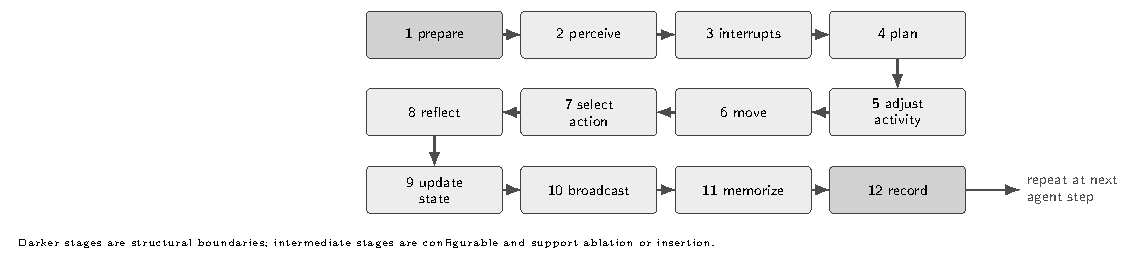
\includegraphics[width=\linewidth]{agent_lifecycle.pdf}
  \caption{The configured default agent-step pipeline.  The first and last
  stages are structural boundaries; intermediate stages may be omitted or
  replaced through configuration.  Domain inputs also arrive through direct
  calls, event-bus contribution points, plugin lifecycle hooks, and a player
  intervention queue; the diagram is a control-flow account rather than a
  claim that every subsystem is a plugin.}
  \label{fig:agent-lifecycle}
\end{figure}

\begin{figure}[t]
  \centering
  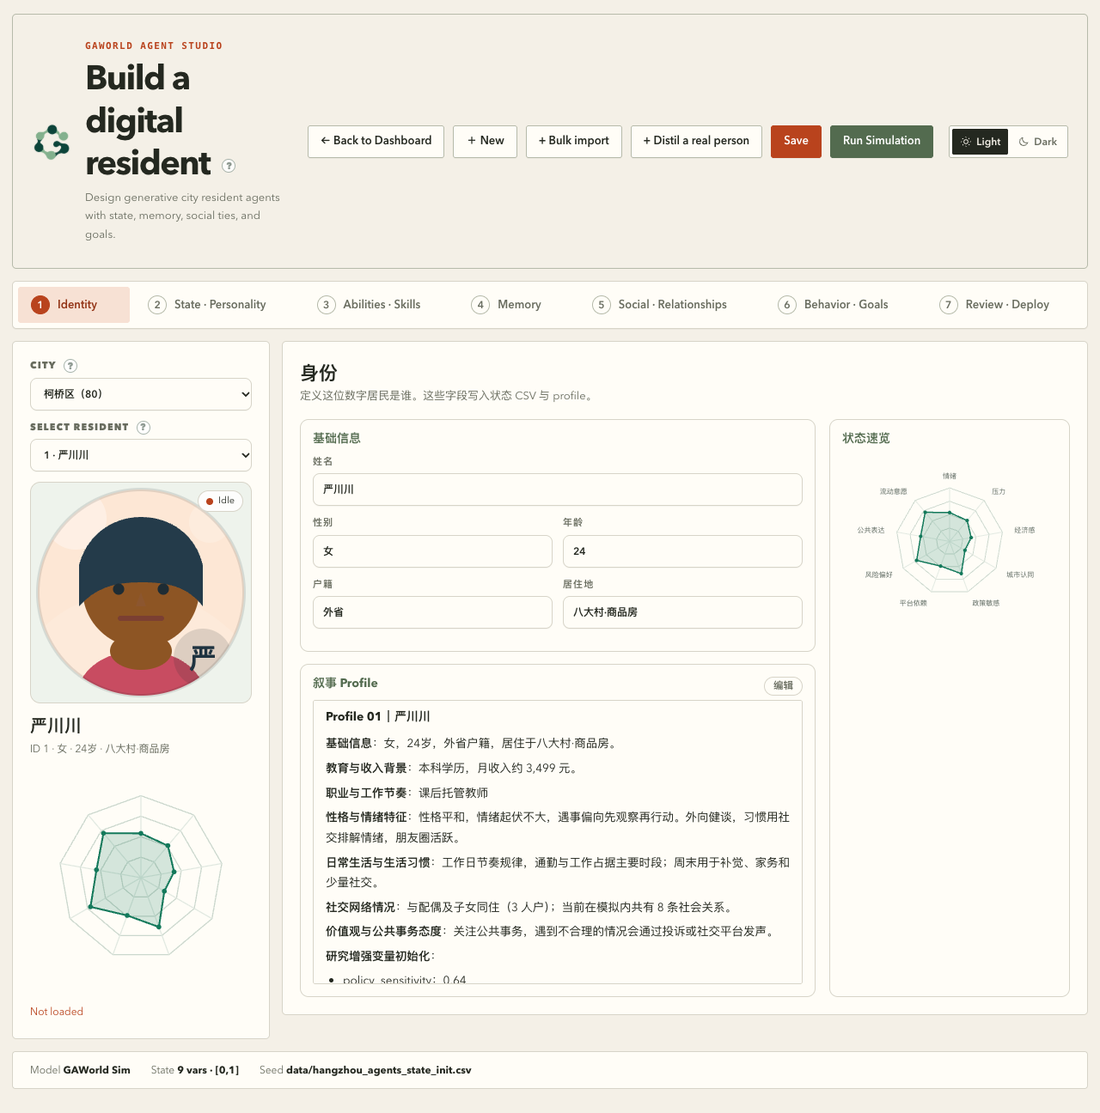
\includegraphics[width=\linewidth]{en_02_studio.png}
  \caption{The Agent Studio.  The seven-step tab at the top
  (\emph{Identity, State \& Personality, Abilities \& Skills, Memory,
  Social \& Relationships, Behavior \& Goals, Review \& Deploy}) maps one
  to one onto the seven sections of an Agent Studio session.  The left
  column selects the city and the resident; the right radar plots the
  normalized state across nine axes (activity, public-expression,
  pressure, economic sense, city recognition, policy sensitivity,
  risk preference, platform dependence, mobility intent).  The
  \emph{Profile} pane is the sourced-portrait view; the persona
  distillation module can write a similar portrait from a name or a
  URL through the \emph{Distill a real person} button on the top right.}
  \label{fig:agent-studio}
\end{figure}

\subsection{Profile seeds, mutable state, and personality}

At construction time, a tabular seed row supplies the identifier, demographic
fields, and initial scalar state, while a Markdown profile supplies descriptive
material such as occupation, daily life, and values.  The current builder
merges these sources into a dictionary containing \texttt{id}, profile fields,
\texttt{state}, an in-memory \texttt{memory} list, \texttt{social\_neighbors},
\texttt{personality} (Big-Five proxies), and \texttt{ext} (per-plugin
namespaces); it then initializes location against the city map and
personality against the configured personality plugin.  The core state includes
affective, socioeconomic, identity, behavioral, and information-exposure
variables.  Additional mechanisms may add namespaced or compatibility fields
during setup and execution.

v2 adds a \emph{personality plugin} that supplies Big-Five-derived proxies
(openness, conscientiousness, extraversion, agreeableness, neuroticism) for
every resident, used by the dynamic-interruption module and by selection
probabilities across the platform.  The plugin's anchors (a deterministic
fallback) and a model-derived overlay (an LLM cache keyed by a profile
signature) coexist; an experimental configuration can select the LLM overlay,
the deterministic anchors, or a custom provider.  The personality module also
maintains a corpus-rewrite pass that compares anchor distributions across
calibrators and warns when one trait dominates a group that the
configuration does not intend to dominate, in the spirit of recent work on
within-group flattening \citep{wang2025flatten}.

The class \texttt{gaworld.core.agent.Agent} is a typed adapter over the
backing dictionary.  It provides properties for identifier, name, state,
memory, schedule, location, attached skill identifiers, and personality
proxies, while dictionary access delegates to the same backing object.
\texttt{view\_as\_agent} therefore introduces no copy, and
\texttt{ensure\_agent\_dict} allows a typed caller to hand the record back to
older helpers.  This is important for incremental migration, but it is not a
fully typed agent schema: many runtime call sites still consume dictionaries,
and arbitrary mechanism-specific fields can still be added.

\subsection{Per-agent directory and persistence}

Persistence extends beyond the in-memory record.  Depending on enabled
features, per-agent directories hold episodic entries, diaries, schedules,
vector-indexed recall material, environmental preferences, private skills,
organization memberships, and travel itineraries.  On a stateful restart,
stored memory is loaded into the agent and can seed retrieval.  The file
boundary makes inputs to later decisions inspectable, although it also means
that reproducibility depends on capturing configuration, external model
behavior, and the complete artifact directory rather than only the seed CSV.

\subsection{The default per-tick path}
\label{sec:lifecycle:pipeline}

The cognition loop is implemented as an ordered \texttt{StagePipeline}.  A
stage receives an agent, a shared per-step dictionary, and the
\texttt{SimContext}.  Hook-visible values retain names such as
\texttt{activity}, \texttt{action}, \texttt{outcome}, and \texttt{reflection};
intermediate values use underscore-prefixed keys.  The default path contains
the following twelve stages, matching v1 with one explicit v2 addition:

\begin{enumerate}[leftmargin=*,label=\arabic*.]
  \item \textbf{prepare} establishes tick-local inputs and emits the pre-step
  boundary;
  \item \textbf{perceive} combines local environment, social, policy, memory,
  and contributed perception sections, including the indoor-room slot that
  names the room the agent is currently occupying;
  \item \textbf{interrupts} considers events that can alter the scheduled
  course, drawing on the dynamic-behavior module and personality proxies;
  \item \textbf{plan} forms the agent's immediate intention in the current
  context;
  \item \textbf{adjust\_activity} reconciles that plan with scheduled and
  interrupted activity;
  \item \textbf{move} resolves travel and updates location, then resolves the
  indoor room that the activity places the agent in (the v2 indoor-room
  hook fires here);
  \item \textbf{select\_action} chooses an action from the available action
  space, optionally mediated by a Controller validator chain;
  \item \textbf{reflect} produces an interpretation of action and outcome;
  \item \textbf{update\_state} applies state, relationship, and organization
  effects;
  \item \textbf{broadcast} exposes eligible communication to other agents or
  a distributed relay, including a player-say channel for human participants;
  \item \textbf{memorize} constructs and stores the tick's experience; and
  \item \textbf{record} appends established logs, state history, Recorder
  events, and visual trace material.
\end{enumerate}

Before the pipeline runs, the outer loop advances the shared Clock, updates
the environment and local occupancy, polls distributed messages when enabled,
and may perform configured information seeking.  After it returns, the
runtime emits \texttt{on\_agent\_post\_step}, allowing mechanisms such as the
intervention, governance, and organizations plugins to compute their own
metrics.  Day-start and day-end events bracket the tick loop; memory
consolidation, governance tallying, and organization-rule resolution are
invoked at the day boundary.  The twelve stages are therefore the agent-step
spine, not the entire simulation lifecycle.

\subsection{Contribution points and compatibility calls}

The EventBus lets a mechanism observe an event, contribute zero or more items,
or filter a value in priority order.  Perception composition is a concrete
example: local context can be assembled by established code while plugins add
bounded text sections without owning the full prompt.  Post-step and day-end
events similarly let policy, economy, skills, interests, organizations, or
governance react at defined boundaries.  Observer failures are logged and
isolated unless strict mode is enabled; stage failures instead propagate
because a missing control-flow stage could silently corrupt state.

Not all inputs use this bus.  Memory recall, environment evolution, and
social-network operations retain direct paths within or around the pipeline.
The Controller now validates structured movement requests and exposes audited
runtime interventions, but it does not mediate every selected action.
Likewise, \texttt{record} writes established artifacts in addition to the
kernel Recorder.  The lifecycle is connected and configurable while retaining
compatibility paths beyond the plugin boundary.

\subsection{Player interventions and the away state}

v2 adds two new first-class inputs to the lifecycle.  A \emph{player
intervention} arrives through the same Controller queue as scheduled events;
its type is one of \texttt{player\_claim}, \texttt{player\_act},
\texttt{player\_say}, or \texttt{player\_release}.  In a single-process
deployment, the intervention enters the local queue; in a multi-node
deployment, the hub routes the intervention to the node that owns the
resident, and the node enqueues it for the next tick.  Either way, the
intervention is then delivered to the agent's \texttt{interrupts} stage
(claim/release affect the lease) or \texttt{perceive} stage (act / say
appear in the next perception), and is recorded in the audit trail.  The
away state is a per-agent \texttt{travel} namespace that holds
\texttt{status}, \texttt{purpose}, \texttt{place}, \texttt{distance\_km},
\texttt{home\_node}, \texttt{depart\_day}, \texttt{return\_day}, and
\texttt{fare}; the agent's \texttt{locations.current} is rewritten to
\texttt{away (\textit{place})} so that occupancy calculations exclude the
agent without losing the round-trip.  Coming home restores
\texttt{locations.current} from \texttt{home\_node} so that travel time and
fare are computed against a real node rather than a label.

\subsection{Configuration and ablation semantics}

The stage order is read from \texttt{CONFIG["pipeline"]["agent\_step"]}.
Entries may name built-in stages or importable callables; a custom callable
can also receive a display name.  Unresolvable entries are skipped with a
warning, and an empty resolved pipeline is rejected.  Downstream built-ins
generally read absent step values defensively, which supports mechanism
ablations, but \texttt{prepare} and \texttt{record} are intended as
structural boundaries.  Changing order or removing a stage can change
semantics and artifact completeness.  The configuration surface enables
controlled system experiments; it does not guarantee that every permutation
is meaningful or behavior-preserving.
